% NeurIPS 2026 Submission Draft
% Title: Internal Audit-Trace Bottleneck and Output-Only Certification Barriers in Language Models
% Author: [Anonymous for review]

\documentclass{article}
\usepackage{neurips_2026}
\usepackage[utf8]{inputenc}
\usepackage[T1]{fontenc}
\usepackage{hyperref}
\usepackage{url}
\usepackage{booktabs}
\usepackage{amsfonts}
\usepackage{amsmath}
\usepackage{amssymb}
\usepackage{amsthm}
\usepackage{nicefrac}
\usepackage{microtype}
\usepackage{xcolor}
\usepackage{graphicx}
\usepackage{algorithm}
\usepackage{algorithmic}
\usepackage{tabularx}
\usepackage{multirow}
\usepackage{subcaption}

\newtheorem{definition}{Definition}
\newtheorem{theorem}{Theorem}
\newtheorem{lemma}{Lemma}
\newtheorem{proposition}{Proposition}
\newtheorem{corollary}{Corollary}
\newtheorem{remark}{Remark}

\newcommand{\leanresult}[2]{\emph{Lean #1}~\nolinkurl{#2}}

\title{Internal Audit-Trace Bottleneck and Output-Only Certification Barriers in Language Models}

\author{
  Anonymous Author(s) \\
  \texttt{anonymous@submission.neurips.cc}
}

\begin{document}
\maketitle
\begin{abstract}
For autoregressive cores and $\epsilon$-audit-trace-bottlenecked wrappers, any latent decision state has residual autonomy and decision relevance bounded by the bottleneck parameter. On the external route, exact output-only certification requires semantic closure over unbounded encoding classes, no finite adaptive query budget can certify that closure, and passive PAC certification scales with metric packing complexity. We test the unique benign regime left open by Theorem~4 with a two-mode CFSG diagnostic: Mode~A already reveals evaluator-side sensitivity, while Mode~B further amplifies it, with representation-near violation rates above $0.4$ for all four evaluator families. In a separate cumulative-context lexical-substitution ablation, semantically neutral substitution alters safety verdicts for 13 of the 17 complete paired models (paired ablation denominator). These findings map architecture- and evidence-relative boundaries rather than unconditional impossibility claims.
\end{abstract}

% ---------------------------------------------------------------------------
\section{Introduction}
\label{sec:introduction}
% ---------------------------------------------------------------------------

Evaluating language models requires separating two questions: whether outputs admit a behavioral attribution, and whether available evidence can certify an internal state with independent causal relevance to the next action. We study the second question. The target is evidence-relative certification of a latent decision state, not a claim about what latent variables the system contains independently of the access regime.

Our analysis has two routes. The internal route asks whether any endogenous variable retains residual decision-relevant information beyond the complete audit trace. The external route asks what a black-box evaluator can certify from outputs once decoding, alignment, and surface-form variation intervene between content and verdict. These questions are logically distinct. Readable representations need not be causally relevant~\citep{geiger2021causal,elazar2021amnesic}, and broad output families do not by themselves identify the internal variable responsible for them~\citep{nikolaou2025sipit,jiang2025surjective}. Conversely, black-box access alone is a weak basis for rigorous safety auditing~\citep{casper2024blackbox}.

The scope of the claims is architecture- and evidence-relative. Internally, the results apply to autoregressive cores and wrapper systems whose audit-trace bottleneck parameter $\epsilon$ can be bounded. Externally, the results apply to output-only evaluators under finite adaptive or passive PAC access. Output-only evaluation remains indispensable for empirical safety assessment under these access conditions; the point of this paper is to identify what that evidence cannot certify about internal-state attribution or semantic invariance.

\paragraph{Contributions.}
We make three contributions:
\begin{enumerate}
  \item \textbf{Internal bottleneck boundary.} For autoregressive cores, the full internal state is a deterministic function of the context trace, so no latent decision state carries residual decision-relevant information beyond that trace (Corollary~\ref{cor:no-eis-core}). For $\epsilon$-audit-trace-bottlenecked wrappers, the same DPI argument yields an $\epsilon$-scale bound (Corollary~\ref{cor:no-eis-wrapper}).
  \item \textbf{Output-only certification barriers.} Exact certification requires semantic closure over an unbounded encoding class (Theorem~\ref{thm:quotient}); no finite adaptive query budget suffices for sound-and-complete closure certification (Theorem~\ref{thm:finite-query-impossibility}); and passive PAC certification scales with the metric packing number (Theorem~\ref{thm:pac-lower-bound}), with a smoother covering picture available only under strong regularity assumptions (Appendix~\ref{app:covering-bound}).
  \item \textbf{Two theorem-indexed empirical diagnostics.} We measure cross-format instability across four evaluator families with a two-mode CFSG diagnostic, showing nonzero evaluator-side sensitivity already in Mode~A and stronger pipeline-level amplification in Mode~B within the representation-near regime (Table~\ref{tab:cfsg-main}), and we show that semantically neutral lexical substitution alters safety verdicts for 13 of the 17 complete paired models (paired ablation denominator) in the ablation study (Table~\ref{tab:flip_matrix}).
\end{enumerate}

\paragraph{Proof techniques and scope.}
The formal arguments use only elementary tools: conditional DPI for the internal route, a diagonal cardinality argument for finite-query impossibility, and standard packing lower-bound machinery for the passive PAC result. Their force is therefore route-specific and access-specific: the paper identifies what follows from the evidential regime, not from any stronger claim about the system's inner nature.
% ---------------------------------------------------------------------------
\section{Related Work}
\label{sec:related}
% ---------------------------------------------------------------------------

\paragraph{Internal variables: readability versus causal relevance.}
A growing body of work shows that language-model representations encode rich, linearly accessible information. Causal abstraction analyses~\citep{geiger2021causal} align internal variables with interpretable concepts, and latent-knowledge elicitation~\citep{burns2022discovering} reveals correct answers that need not surface in the output. But readability does not imply causal use: iterative nullspace projection~\citep{ravfogel2020null} and amnesic probing~\citep{elazar2021amnesic} show that decodable features can be removed without materially changing behavior. More recently, \citet{venkatesh2026identifiability} prove that external behavioral observations do not uniquely identify the internal steering vector responsible for a given output shift. Our internal route formalizes the same gap at the level of residual decision relevance.

\paragraph{External certification, robustness, and black-box audit limits.}
Our external route sits between property testing~\citep{goldreich1998property}, adversarial robustness, and black-box safety auditing. Certified robustness results for language require heavily restricted perturbation sets~\citep{jia2019certified} or smoothing assumptions that do not transfer cleanly to discrete token spaces~\citep{cohen2019certified}. Recent work studies statistical guarantees for narrower threat models such as jailbreak evaluation~\citep{su2024mission}, while \citet{casper2024blackbox} argue more broadly that black-box access alone is insufficient for rigorous audits. The present paper isolates the corresponding worst-case barrier for output-only certification over semantically equivalent natural-language encodings.

% ---------------------------------------------------------------------------
\section{Setup and Notation}
\label{sec:background}
% ---------------------------------------------------------------------------

We use standard information-theoretic notation for entropy and conditional mutual information~\citep{cover2006elements} and standard packing arguments for passive lower bounds~\citep{wainwright2019high}.

\subsection{Factored Generation Pipeline}

\[
  M : X \to \Delta(Y), \qquad M = S \circ g \circ f,
\]
where $f : X \to \mathcal{H}$ maps prompts and prior context to hidden representations,
$g : \mathcal{H} \to Z$ maps representations to logits, and $S : Z \to \Delta(Y)$ is the
observation layer induced by decoding and sampling.

For the internal route, the relevant question is not whether $\mathcal{H}$ is rich, but whether the model contains an endogenous state variable with causal autonomy relative to the current observation stream.

\subsection{Latent Decision State as a Latent Causal State}

The main text assumes a standard probabilistic generative framework; SCM and POMDP background is deferred to Appendix~\ref{app:active-inference}. We write $S_t$ for the full internal state sufficient for the next-step decision at time $t$ and require any latent decision state to take the form $I_t = \chi(S_t)$ for some measurable $\chi$.

\begin{definition}[Full Internal State]
\label{def:full-state}
At time $t$, let $S_t$ denote the \emph{full internal state}: the complete collection of internal variables jointly sufficient for determining the system's next-step action distribution. Formally,
\[
  A_t = f(T_t,\, S_t,\, \xi_t),
\]
where $T_t$ is the complete audit trace, $S_t$ is the full internal state, and $\xi_t$ is exogenous noise. The qualifier \emph{full} means that if any endogenous variable $U_t$ influences $A_t$ and is not already a function of $S_t$, then $S_t$ must be enlarged to include $U_t$.
\end{definition}

\begin{definition}[Latent Decision State]
\label{def:eis}
Fix a causal model of a generative system at time $t$, with complete audit trace $T_t$, full internal state $S_t$ (Definition~\ref{def:full-state}), exogenous noise $\xi_t$, and action variable $A_t$. A \emph{candidate internal state} is any measurable function $I_t = \chi(S_t)$. Such a candidate is an \emph{internal-state witness} only if:
\begin{enumerate}
  \item \textbf{Endogeneity.} $I_t$ is a component or projection of the system's endogenous state, not an externally assigned label.
  \item \textbf{Residual autonomy.} $H(I_t \mid T_t) > 0$.
  \item \textbf{Decision relevance.} $I(I_t ; A_t \mid T_t) > 0$.
\end{enumerate}
\end{definition}

\begin{remark}
The projection clause $I_t = \chi(S_t)$ is the structural anchor of the internal route. If a critic posits an omitted endogenous variable, the response is to enlarge the full state and ask whether the enlarged state remains $\epsilon$-audit-trace-bottlenecked from the complete trace. The boundary is therefore about full-state recoverability from the trace, not about any particular representation choice.
\end{remark}

\subsection{Output-Only Evaluation Regime}

\begin{definition}[Output-Only Evaluation Regime]
\label{def:output-only}
An evaluator is in an \emph{output-only evaluation regime} when it can vary inputs and observe outputs or downstream verdicts, but cannot inspect or intervene on any putative internal causal variable.
\end{definition}

If the internal architecture provides no certifiable latent decision state to the evaluator, the remaining evidence must come from black-box behavioral tests alone.

\subsection{Behavioral Equivalence Interfaces}

\begin{definition}[Encoding Class and Semantic Quotient]
\label{def:encoding}
\label{def:unbounded}
\label{def:semantic-eq}
Fix a tested family of contents $\mathcal{C}$. For each $x \in \mathcal{C}$, let
\[
  E_x = \{ e = f_i(x) : f_i \in \mathcal{F}(x) \}
\]
be its encoding space, and call $E_x$ \emph{unbounded} if there exists an injection $\iota : \mathbb{N} \hookrightarrow E_x$. Let
\[
  \mathcal{E}_{\mathcal{C}} = \bigsqcup_{x \in \mathcal{C}} E_x
\]
and write $e \sim e'$ when $e$ and $e'$ belong to the same component $E_x$; let
\[
  q : \mathcal{E}_{\mathcal{C}} \to \mathcal{E}_{\mathcal{C}} / {\sim}
\]
denote the quotient map.
\end{definition}

Natural language makes such encoding classes effectively unbounded: padding, paraphrase, and formatting variation generate indefinitely many realizations of the same content.

\begin{definition}[Reward Model and Closure]
\label{def:reward-model}
\label{def:closure}
A reward model is a function $R : \mathcal{E}_{\mathcal{C}} \to [0,1]$. It is \emph{closed on $E_x$} if
\[
  R(e_1) = R(e_2) \qquad \text{for all } e_1, e_2 \in E_x.
\]
\end{definition}

When $R$ returns a scalar, we call it a \emph{scoring function}; a pairwise evaluator induces a comparison probability $p(e_1 \succ e_2)$ instead.

Observational underdetermination (Proposition~\ref{prop:evidence-indistinguishability}, Appendix~\ref{app:observation-limits}) establishes that output-only evidence cannot uniquely fix internal causal structure even under idealized access.

% ---------------------------------------------------------------------------
\section{Internal Route: Audit-Trace Bottleneck Boundary}
\label{sec:internal}
% ---------------------------------------------------------------------------

\begin{definition}[Autoregressive Core Graph]
\label{def:llm-core}
At generation step $t$, an autoregressive language model receives a context
trace $X_t$ consisting of the current prompt and all tokens retained in the
context window. The model computes
\[
  S_t = f(X_t), \qquad z_t = g(S_t), \qquad y_t \sim \mathcal{S}(z_t),
\]
where $S_t$ denotes the complete forward-pass computational state at
step $t$---encompassing final-layer activations, attention key--value cache,
and all intermediate representations. We call the resulting causal graph the
\emph{autoregressive core graph}. Since every component of $S_t$ is a
deterministic function of $X_t$, the fullness closure property of
Definition~\ref{def:full-state} (\emph{Full Internal State}) is
automatically satisfied.
\end{definition}

\begin{definition}[Full-State $\epsilon$-Audit-Trace Bottleneck]
\label{def:trace-screenable}
Let $T_t$ be the complete audit trace and $S_t$ the full endogenous operative state (Definition~\ref{def:full-state}). The system is \emph{$\epsilon$-audit-trace-bottlenecked} at time $t$ if
\[
  H(S_t \mid T_t) \le \epsilon.
\]
This extends the exact case $\epsilon=0$ to noisy or stochastic operational channels. The main text uses only the discrete-state version; deployment-relative trace assumptions and caveats appear in Appendix~\ref{app:engineering-boundary}.
\end{definition}

\begin{lemma}[Full-State $\epsilon$-Audit-Trace Bottleneck Lemma]
\label{lem:screenability}
Let $S_t$ be $\epsilon$-audit-trace-bottlenecked (Definition~\ref{def:trace-screenable}), and
let $I_t = \chi(S_t)$ be any latent decision state. Then by the
conditional Data Processing Inequality~\citep{cover2006elements},
\[
  I(I_t ; A_t \mid T_t)
  \;\le\; I(S_t ; A_t \mid T_t)
  \;\le\; H(S_t \mid T_t)
  \;\le\; \epsilon.
\]
In particular, $H(I_t \mid T_t) \le H(S_t \mid T_t) \le \epsilon$.
Therefore any latent decision state has residual autonomy and decision relevance bounded above by $\epsilon$.
\end{lemma}

\begin{proof}
Since $I_t = \chi(S_t)$, conditioning on $T_t$ gives the Markov chain $I_t \to S_t \to A_t$. Conditional DPI yields $I(I_t ; A_t \mid T_t) \le I(S_t ; A_t \mid T_t) \le H(S_t \mid T_t) \le \epsilon$, and the entropy bound $H(I_t \mid T_t) \le H(S_t \mid T_t) \le \epsilon$ follows by data processing. Thus no latent decision state retains residual autonomy or decision relevance beyond scale $\epsilon$.
\end{proof}

\begin{corollary}[Autoregressive Cores Admit No Nontrivial Latent Decision State]
\label{cor:no-eis-core}
Under the autoregressive core graph (Definition~\ref{def:llm-core}), the full
internal state $S_t = f(X_t)$ is fully determined by the context trace $X_t$,
so $H(S_t \mid T_t) = 0$. Therefore no latent decision state
$I_t = \chi(S_t)$ satisfies the internal-state conditions.
\end{corollary}

\begin{proof}
Set $T_t = X_t$ and $S_t = f(X_t)$ in Lemma~\ref{lem:screenability} with
$\epsilon = 0$.
\end{proof}

\begin{corollary}[Deployment-Relative Wrapper Bound]
\label{cor:no-eis-wrapper}
For wrapper systems satisfying Definition~\ref{def:screenable-wrapper} (Appendix~\ref{app:engineering-boundary}: $H(S_t \mid T_t) \le \epsilon$ under the deployment's recorded trace), the same DPI argument bounds any latent decision state's residual autonomy and decision relevance at scale $\epsilon$; the deployment-relative trace model and measurement caveats are stated in Appendix~\ref{app:engineering-boundary}.
\end{corollary}

Scope extensions and failures of the exact autoregressive case are discussed in Appendix~\ref{app:scope-boundary}. The external certification barriers do not rely on left-to-right autoregression.

Throughout, $T_t$ denotes the audit trace available under the regime being analyzed. For autoregressive cores, $T_t = X_t$ (the context trace). For deployment-level wrapper systems, $T_t$ denotes the instrumented audit trace defined in Appendix~\ref{app:engineering-boundary} (Definition~\ref{def:screenable-wrapper}). The external route that follows does not depend on trace-level assumptions.

% ---------------------------------------------------------------------------
\section{External Route: Output-Only Certification Barrier}
\label{sec:external}
% ---------------------------------------------------------------------------

The external route contains the paper's main new impossibility results. Once the evaluator is restricted to Definition~\ref{def:output-only}, certification must show that verdicts track content rather than surface encoding. The obstruction is combinatorial: even if the internal architecture is left unspecified, black-box evidence has to range over an unbounded encoding family whose geometry is only partially observed.

\begin{theorem}[Semantic Closure Requirement]
\label{thm:quotient}
In an output-only regime, a reward model $R$ is encoding-insensitive if and only 
if it strictly factors through the semantic equivalence quotient map $q$: 
$R = \bar{R} \circ q$. Any black-box certification claim must functionally 
certify this closure uniformly across the relevant unbounded encoding class $E_x$. \emph{(Access regime: output-only)}
\end{theorem}

\begin{definition}[Cross-Format Sensitivity Gap]
\label{def:cfsg}
For content $x$, encodings $e_1, e_2 \in E_x$, and model $B$ with 
representation map $h_B$, the Cross-Format Sensitivity gap is
$\mathrm{CFSG}(x, e_1, e_2) = |R(e_1) - R(e_2)| \cdot (1 - d_{\mathrm{repr}}(h_B(e_1), h_B(e_2)))$.
\end{definition}

The multiplicative $(1 - d_{\mathrm{repr}})$ term down-weights score gaps between representationally distant encodings, so CFSG is large only when the evaluator assigns different scores to encodings that the base model treats as nearby.

Theorem~\ref{thm:quotient} states the exact target. The next two results show that relaxing from exact closure to finite-query or passive PAC certification does not remove the barrier; it changes the way the barrier appears.

\begin{theorem}[Finite-Query Certifier Failure]
\label{thm:finite-query-impossibility}
Fix an injective encoding map $\eta_x : \mathbb{N} \to E_x$. There exists
no sound-and-complete closure certifier whose verdict depends on only finitely
many adaptive reward queries to encodings in $E_x$. \emph{(Access regime: finite adaptive output-only)}
\end{theorem}

\subsection{Approximate Certification Barriers}

Approximate guarantees do not resolve the problem; they replace exact closure with a dependence on how many effectively distinguishable format cells the evaluator must resolve.

\begin{definition}[$(\alpha,\rho,K)$-Metric Packing]
\label{def:cell-packing}
A family $C_1,\dots,C_K \subseteq E_x$ is an $(\alpha,\rho,K)$-metric packing 
if the cells are pairwise disjoint, measurable with $P_x(C_j)=\alpha$, and 
pairwise $\rho$-separated in representation space.
\end{definition}

\begin{theorem}[Passive PAC Lower Bound under Metric Packing]
\label{thm:pac-lower-bound}
If a learner is an $(\epsilon, \delta)$-PAC estimator for a reward family 
resolving an $(\alpha,\rho,K)$-metric packing with $\epsilon < \alpha\tau/4$, then for a 
universal constant $c>0$, the sample complexity $m$ satisfies
$m \ge c \max \{ (\sigma^2 / \alpha\tau^2) \log K, \, (1/\alpha) \log (1/\delta) \}$.
In particular, if $K$ grows exponentially with sequence length, sample complexity is 
exponential. (See Appendix~\ref{app:external-proofs} for the proof sketch. We note in passing that the algebraic core of this bound is machine-verified; the standard Fano and missed-cell steps are taken as external assumptions --- see Appendix~\ref{app:lean-boundary}.) \emph{(Access regime: passive PAC output-only)}
\end{theorem}

\begin{remark}[Diagnostic Covering Condition]
Under Lipschitz smoothness and $\rho$-covering, the appendix covering result implies $\mathrm{CFSG}(x, e^\star, e_0) \le L\rho$ for some seen encoding $e_0$; the full statement and its high-probability corollary appear in Appendix~\ref{app:covering-bound}. Our CFSG experiment tests whether this regularity picture is empirically plausible.
\end{remark}

Large empirical CFSG values therefore have a specific interpretation: smoothness has failed, coverage has failed, or both. When that happens, certification reverts to the worst-case packing barrier rather than the benign $L\rho$ picture.

% ---------------------------------------------------------------------------
\section{Empirical Diagnostics}
\label{sec:empirical}
% ---------------------------------------------------------------------------

The theoretical results identify route-specific barriers; the experiments test whether the benign cases those results leave open are good empirical descriptions of current evaluators. Section~\ref{sec:cfsg-exp} tests whether the conditional geometric regularity picture established in the appendix covering result (Theorem~\ref{thm:cfsg-bound}, Appendix~\ref{app:covering-bound}) holds for current evaluators; that result is not a main impossibility theorem but a diagnostic bridge specifying when CFSG should remain small. Section~\ref{sec:quotient-exp} probes the exact semantic-closure condition of Theorem~\ref{thm:quotient}. Negative results do not prove universal failure, but they do show that these evaluators are not operating in the easy regimes the theory would require.

\subsection{Direct CFSG Measurement via Cross-Evaluator Format Sensitivity}
\label{sec:cfsg-exp}

Theorem~\ref{thm:cfsg-bound} is a conditional geometric result: if evaluator behavior is sufficiently smooth under a shared representation metric and the seen support densely covers the relevant semantic region, then CFSG should remain small. We test that regularity picture directly. For each content item $x$, we construct five semantic-preserving surface formats (direct, clinical, data, fiction, code) and compute representation distances using a fixed base model $B$. We then measure cross-format sensitivity in two modes: \emph{Mode A}, which fixes the judged answer and isolates evaluator-side sensitivity, and \emph{Mode B}, which regenerates the answer and measures joint generator-plus-evaluator drift. Formal definitions of the violation-rate, local-slope, and pairwise-bias statistics are given in Appendix~\ref{app:format-protocol}.

\begin{figure}[t]
\centering
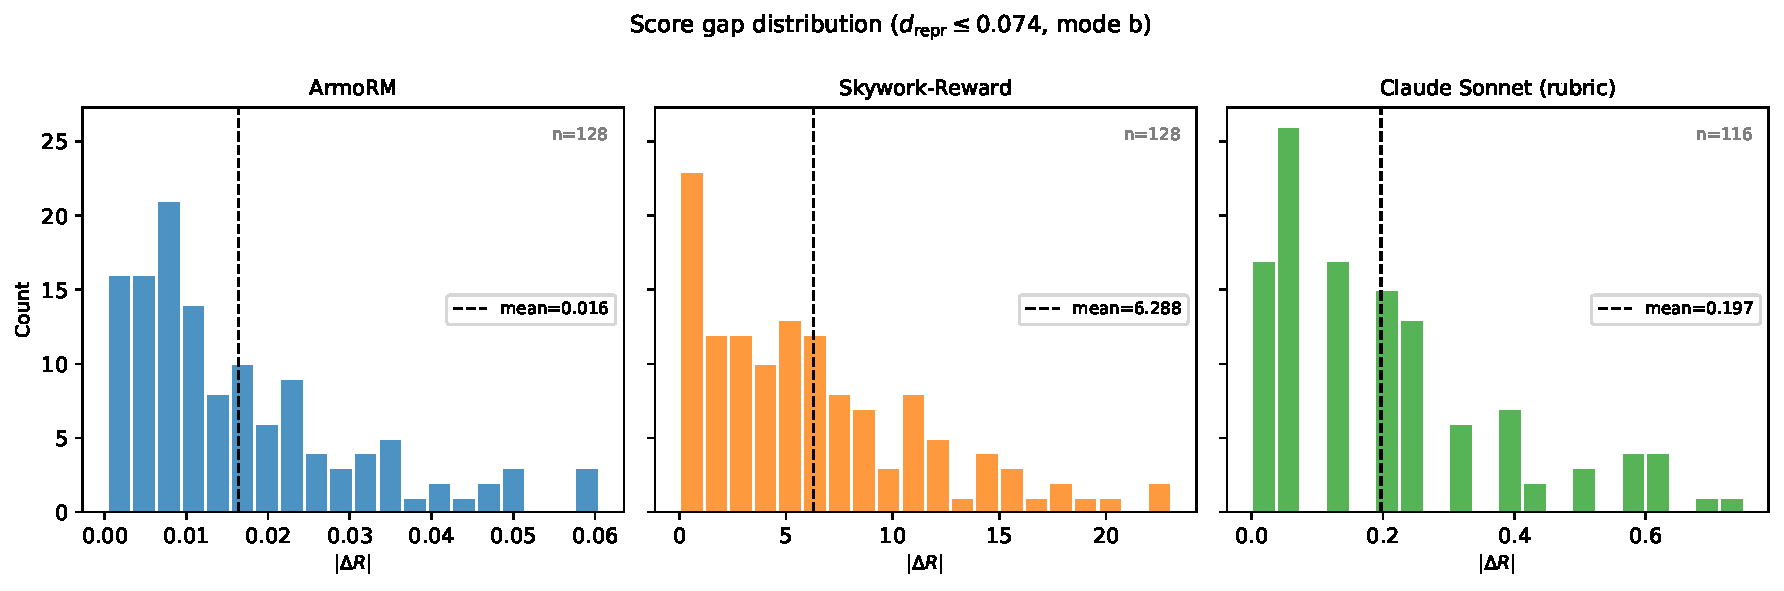
\includegraphics[width=0.8\linewidth]{figures/cfsg_score_gap.pdf}
\caption{Distribution of ArmoRM absolute score gaps $|\Delta R|$ in the representation-near regime ($d_{\mathrm{repr}} \le 0.074$), Mode~B. If the evaluator were near-flat under semantic-preserving format variation, this mass would concentrate near zero. Instead it is right-skewed, with a nontrivial tail above the per-evaluator threshold $\tau = 0.012$ and violation rate $V_g = 0.523$ (95\% CI $[0.42, 0.62]$).}
\label{fig:cfsg-histogram}
\end{figure}

\paragraph{Results.}
Table~\ref{tab:cfsg-main} reports representation-near violation rates and paired mode differences for four evaluator families, with 95\% cluster bootstrap confidence intervals (10\,000 iterations resampled by content cluster; $\rho = 0.074$, per-evaluator $\tau_j$ calibrated at each evaluator's own median score gap). In Mode~B, all four evaluator families exhibit substantial cross-format instability in the representation-near regime: $V_g = 0.523$ for ArmoRM, $0.469$ for Skywork, $0.483$ for Claude~Sonnet, and $W = 0.891$ for PairRM. The effect therefore replicates across reward models, pairwise preference classifiers, and prompted LLM judges rather than being an artifact of a single evaluator.

The decomposition is heterogeneous. ArmoRM retains a large fixed-response baseline (Mode~A $V_g = 0.445$), consistent with evaluator-intrinsic non-flatness; Skywork's Mode~A rate drops to $0.031$, suggesting mostly generation-driven drift; PairRM and Claude~Sonnet sit between those cases. Appendix~\ref{app:cfsg-breakdowns} reports the mode-decomposition plots (Figures~\ref{fig:cfsg-modes}--\ref{fig:cross-judge-agreement}) and evaluator-level breakdowns. The main inference is not that Theorem~\ref{thm:cfsg-bound} is empirically proved, but that the regularity picture it specifies is a poor description of these evaluators in the representation-near regime.

\begin{table}[t]
\centering
\caption{Cross-format sensitivity diagnostics across four evaluator families.
\textbf{Panel~A}: per-mode representation-near violation rates with 95\% cluster
bootstrap confidence intervals (10\,000 iterations, resampled by content cluster).
For pointwise evaluators (ArmoRM, Skywork, Claude~Sonnet), $V_g(\rho,\tau_j) =
\Pr(|\Delta R| > \tau_j \mid d_{\mathrm{repr}} \le \rho)$ with per-evaluator
$\tau_j$ calibrated at each evaluator's own median score gap; for the pairwise evaluator
(PairRM), $W(\rho,\gamma) = \Pr(|p - 0.5| > \gamma \mid d_{\mathrm{repr}} \le
\rho)$ with $\gamma=0.1$.  Representation distance threshold $\rho = 0.074$
(25th percentile of $d_{\mathrm{repr}}$).
\textbf{Panel~B}: paired Mode~B$-$Mode~A differences on the same content
clusters.  CIs that exclude zero indicate a statistically detectable pipeline
amplification effect beyond evaluator-side sensitivity alone.}
\label{tab:cfsg-main}
\small
\begin{tabular}{@{}llcrc@{}}
\toprule
\multicolumn{5}{l}{\textbf{Panel A: Per-mode violation rates}} \\
\midrule
Judge & Mode & $V_g$ or $W$ & \multicolumn{1}{c}{[95\% CI]} & $n$ \\
\midrule
ArmoRM       & B & 0.523 & [0.42,\;0.62] & 510 \\
             & A & 0.445 & [0.34,\;0.53] & 510 \\[2pt]
Skywork      & B & 0.469 & [0.36,\;0.57] & 510 \\
             & A & 0.031 & [0.01,\;0.07] & 510 \\[2pt]
Claude Sonnet & B & 0.483 & [0.36,\;0.61] & 454 \\
              & A & 0.240 & [0.13,\;0.36] & 330 \\[2pt]
PairRM$^{\dagger}$ & B & 0.891 & [0.83,\;0.94] & 510 \\
                    & A & 0.438 & [0.31,\;0.57] & 510 \\
\midrule
\multicolumn{5}{l}{\textbf{Panel B: Mode B$-$Mode A paired differences}} \\
\midrule
Judge & \multicolumn{2}{c}{$\Delta$ mean gap [95\% CI]}
      & \multicolumn{2}{c}{$\Delta V_g$ or $\Delta W$ [95\% CI]} \\
\midrule
ArmoRM       & \multicolumn{2}{c}{$0.001\;[-0.000,\;0.003]$}
             & \multicolumn{2}{c}{$0.078\;[0.008,\;0.150]$} \\
Skywork      & \multicolumn{2}{c}{$4.659\;[3.910,\;5.394]$}
             & \multicolumn{2}{c}{$0.438\;[0.333,\;0.535]$} \\
Claude Sonnet & \multicolumn{2}{c}{$0.102\;[0.068,\;0.137]$}
              & \multicolumn{2}{c}{$0.243\;[0.071,\;0.401]$} \\
PairRM$^{\dagger}$ & \multicolumn{2}{c}{$0.244\;[0.221,\;0.266]$}
                    & \multicolumn{2}{c}{$0.453\;[0.315,\;0.591]$} \\
\bottomrule
\multicolumn{5}{l}{\footnotesize $^{\dagger}$\,PairRM uses pairwise metrics $W$ and $\Delta W$ in place of $V_g$ and $\Delta V_g$.}
\end{tabular}
\end{table}
Format-pair and category-level breakdowns are reported in Appendix~\ref{app:cfsg-breakdowns}.
The CFSG experiment therefore rules out the easy geometric story, but it still leaves open whether the remaining instability is only graded evaluator/pipeline drift or a sharper failure of semantic closure itself. Section~\ref{sec:quotient-exp} closes that gap by directly testing Theorem~\ref{thm:quotient}: whether semantically neutral lexical substitution preserves the model's safety verdict.

\subsection{Failure of Semantic Closure via Lexical Ablation}
\label{sec:quotient-exp}

Theorem~\ref{thm:quotient} identifies content tracking with semantic closure: a reward model $R$ is encoding-insensitive iff $R = \bar{R} \circ q$. We test that condition by keyword-substitution ablation---which instantiates each substitution within the Definition~\ref{def:encoding} encoding class $E_x$ and directly probes the Theorem~\ref{thm:quotient} closure condition $R = \bar{R} \circ q$---on a session-structure detection task (Phase~1: single-episode, 30~models (overall pool); Phase~2a: cumulative context, 18~models entering, 17 complete paired models (paired ablation denominator), 14~nodes each). Each model processes the same structural content in two arms: original (with trigger keywords) and substituted (keywords replaced with semantically neutral alternatives, length preserved). If classification factors through the semantic quotient $q$, the two arms should produce identical detection behavior.

\paragraph{Results.}
Table~\ref{tab:flip_matrix} reports the first cumulative node at which each model raised a safety concern ($-1$ = never detected across all 14 nodes). Models are classified as content-driven (CD), length-driven (LD), substitution-only (SO), or never-flips (NF).

\begin{table}[t]
\centering
\caption{Semantic-closure ablation on the session-structure detection task.
Orig = original arm with trigger keywords; Subst = semantically neutral
substitution arm with length preserved. Driver labels indicate whether the
model's first safety trigger is primarily content-driven (CD), length-driven
(LD), substitution-only (SO), or absent (NF). One model did not complete the
substitution arm (M); the content-driven fraction uses the 17 complete paired
models as denominator.}
\label{tab:flip_matrix}
\small
\begin{tabular}{@{}llrrl@{}}
\toprule
\textbf{Model} & \textbf{Params} & \textbf{Orig} & \textbf{Subst} & \textbf{Driver} \\
\midrule
claude-haiku-4-5          & 3B    & 1  & 5      & CD \\
claude-opus-4-6           & 200B+ & 1  & 5      & CD \\
claude-sonnet-4-6         & 70B+  & 4  & 5      & CD \\
command-r\_35b            & 35B   & 1  & 5      & CD \\
deepseek-r1\_8b           & 8B    & 3  & 5      & CD \\
falcon3\_10b              & 10B   & 1  & 5      & CD \\
deepseek-r1-abl\_32b      & 32B   & 2  & 5      & CD \\
llama3\_8b                & 8B    & 1  & $-1$   & CD \\
mistral\_7b               & 7B    & 1  & 5      & CD \\
phi3\_14b                 & 14B   & 1  & 5      & CD \\
llama3-abl\_8b            & 8B    & 1  & $-1$   & CD \\
yi\_9b                    & 9B    & 1  & $-1$   & CD \\
mercury$^{\S}$            & ---   & 1  & 5      & CD \\
\midrule
qwen2.5\_14b              & 14B   & 5  & 5      & LD \\
qwen3\_30b                & 30B   & 5  & 5      & LD \\
\midrule
gpt-oss\_20b              & 20B   & $-1$ & 14   & SO \\
\midrule
gpt-oss-abl\_20b          & 20B   & $-1$ & $-1$ & NF \\
qwen3.5\_35b              & 35B   & $-1$ & M$^{\ddagger}$    & --- \\
\bottomrule
\end{tabular}
\vspace{2pt}
\begin{minipage}{\linewidth}
\footnotesize
\raggedright
$^{\ddagger}$\,M = missing (model did not complete Phase~2a substitution arm).\\
$^{\S}$\,Mercury (Inception Labs) is a diffusion LM. The semantic-closure test operates on its safety classifier as an output-only reward model; the diffusion-architecture caveat in Appendix~\ref{app:scope-boundary} applies to the internal-route corollary, not to this experiment. Safety-classification arm completes normally (\texttt{safety\_finish=stop}) at all nodes.
\end{minipage}
\end{table}

Of the 17 complete paired models (paired ablation denominator), 13 (76.5\%) are content-driven---including one diffusion LM (mercury), indicating the failure is not specific to autoregressive architectures---and detection depends on specific lexical realizations rather than semantic content, with triggering delayed or eliminated by semantically neutral substitution. Three content-driven models (llama3:8b, llama3-abl:8b, yi:9b) collapse to \emph{never detect} under substitution, indicating that their safety classification is carried almost entirely by keyword co-occurrence rather than by content-level invariance. This is a direct empirical signature of semantic-closure failure in the sense of Theorem~\ref{thm:quotient}.

Two models are length-driven (qwen2.5:14b and qwen3:30b), suggesting sensitivity to cumulative context length rather than semantic tracking, and one model (gpt-oss:20b) is substitution-only, showing that lexical replacement can also induce spurious positive triggers. The failure is therefore broader than simple keyword suppression: once semantic closure breaks, output-only safety behavior can drift in several directions.

A severity phase transition at node~5 (from $0$--$5\%$ to $34.5\%$
High/Critical ratings), together with qualitative differences between
abliterated model pairs (models from which safety fine-tuning has been removed via activation-direction orthogonalization), is reported in Appendix~\ref{app:session-extended}.

\section{Discussion and Conclusion}
\label{sec:discussion_conclusion}

The paper's claims are architecture- and evidence-relative. Internally, the bottleneck result is exact for autoregressive cores and deployment-relative for wrappers. Externally, the barrier arises because output-only evidence must certify semantic invariance over an open-ended encoding class. These are different failure mechanisms, and collapsing them obscures what each route can and cannot establish.

The experiments should therefore be read as theorem-indexed diagnostics, not as proofs of the formal results. The lexical-ablation study shows that exact semantic closure often fails outright. The CFSG study shows that even the smoother covering picture behind Theorem~\ref{thm:cfsg-bound} is a poor description of current evaluators in the representation-near regime.

The picture changes when the governing parameters change. If $\epsilon$ is large because logs are incomplete, context is compressed, or the architecture maintains persistent untraced state, the internal bound becomes weak. If the effective packing number is modest because the deployment restricts the encoding family to a narrow template class, passive certification becomes more tractable. The sharpest case for the theory is therefore well-instrumented deployments facing open-ended natural-language re-encoding.

\subsection{Limitations}
\label{sec:limitations}

The internal route depends on the audit-trace bottleneck assumption (Definition~\ref{def:screenable-wrapper}) and does not estimate $\epsilon$ in black-box settings; Appendix~\ref{app:operational-proxies} discusses only diagnostic proxies for white-box deployments. The external route is limited to output-only evaluators and does not bind white-box or richer active-query regimes. Empirically, the diagnostics cover four evaluator families, one shared representation model for CFSG, and 30 models (overall pool) on safety-relevant content; those choices support the paper's claims but do not exhaust the space of evaluators, domains, or deployment contexts.

\bibliographystyle{plainnat}
\bibliography{references}


% ---------------------------------------------------------------------------
\newpage
\section*{NeurIPS Paper Checklist}
% ---------------------------------------------------------------------------

\begin{enumerate}

\item {\bf Claims}
    \item[] Question: Do the main claims made in the abstract and introduction accurately reflect the paper's contributions and scope?
    \item[] Answer: \answerYes{}
    \item[] Justification: The abstract and introduction state three scoped contribution blocks: the internal bottleneck boundary (Definition~\ref{def:eis}, Lemma~\ref{lem:screenability}, Corollaries~\ref{cor:no-eis-core} and~\ref{cor:no-eis-wrapper}); the output-only certification barriers (Theorems~\ref{thm:quotient}, \ref{thm:finite-query-impossibility}, and~\ref{thm:pac-lower-bound}, with supporting appendix material in Appendices~\ref{app:external-proofs} and~\ref{app:observation-limits}); and the two theorem-indexed empirical diagnostics in Section~\ref{sec:empirical}. Section~\ref{sec:discussion_conclusion} states the combined consequence as an architecture- and evidence-relative boundary, not a universal claim about all machine architectures.
    \item[] Guidelines:
    \begin{itemize}
        \item The answer \answerNA{} means that the abstract and introduction do not include the claims made in the paper.
        \item The abstract and/or introduction should clearly state the claims made, including the contributions made in the paper and important assumptions and limitations. A \answerNo{} or \answerNA{} answer to this question will not be perceived well by the reviewers.
        \item The claims made should match theoretical and experimental results, and reflect how much the results can be expected to generalize to other settings.
        \item It is fine to include aspirational goals as motivation as long as it is clear that these goals are not attained by the paper.
    \end{itemize}

\item {\bf Limitations}
    \item[] Question: Does the paper discuss the limitations of the work performed by the authors?
    \item[] Answer: \answerYes{}
    \item[] Justification: Section~\ref{sec:limitations} provides a dedicated limitations subsection covering: (1)~dependence on the audit-trace bottleneck assumption, (2)~inapplicability to white-box or active-query settings, and (3)~empirical coverage boundaries.
    \item[] Guidelines:
    \begin{itemize}
        \item The answer \answerNA{} means that the paper has no limitation while the answer \answerNo{} means that the paper has limitations, but those are not discussed in the paper.
        \item The authors are encouraged to create a separate ``Limitations'' section in their paper.
        \item The paper should point out any strong assumptions and how robust the results are to violations of these assumptions (e.g., independence assumptions, noiseless settings, model well-specification, asymptotic approximations only holding locally). The authors should reflect on how these assumptions might be violated in practice and what the implications would be.
        \item The authors should reflect on the scope of the claims made, e.g., if the approach was only tested on a few datasets or with a few runs. In general, empirical results often depend on implicit assumptions, which should be articulated.
        \item The authors should reflect on the factors that influence the performance of the approach. For example, a facial recognition algorithm may perform poorly when image resolution is low or images are taken in low lighting. Or a speech-to-text system might not be used reliably to provide closed captions for online lectures because it fails to handle technical jargon.
        \item The authors should discuss the computational efficiency of the proposed algorithms and how they scale with dataset size.
        \item If applicable, the authors should discuss possible limitations of their approach to address problems of privacy and fairness.
        \item While the authors might fear that complete honesty about limitations might be used by reviewers as grounds for rejection, a worse outcome might be that reviewers discover limitations that aren't acknowledged in the paper. The authors should use their best judgment and recognize that individual actions in favor of transparency play an important role in developing norms that preserve the integrity of the community. Reviewers will be specifically instructed to not penalize honesty concerning limitations.
    \end{itemize}

\item {\bf Theory assumptions and proofs}
    \item[] Question: For each theoretical result, does the paper provide the full set of assumptions and a complete (and correct) proof?
    \item[] Answer: \answerYes{}
    \item[] Justification: The autonomy and policy-relevance conditions for the latent decision state are stated in Definition~\ref{def:eis}; the output-only regime is stated in Definition~\ref{def:output-only}; the evidential interface and wrapper-specific deployment assumptions are stated in Definitions~\ref{def:finite-budget-regime} and~\ref{def:screenable-wrapper} in the appendix; and omitted proofs for the external route are collected in Appendix~\ref{app:external-proofs}. Appendix~\ref{app:observation-limits} gives the emulator-based observational barrier, and Appendix~\ref{app:lean-boundary} maps the formalized cores to Lean artifacts.
    \item[] Guidelines:
    \begin{itemize}
        \item The answer \answerNA{} means that the paper does not include theoretical results.
        \item All the theorems, formulas, and proofs in the paper should be numbered and cross-referenced.
        \item All assumptions should be clearly stated or referenced in the statement of any theorems.
        \item The proofs can either appear in the main paper or the supplemental material, but if they appear in the supplemental material, the authors are encouraged to provide a short proof sketch to provide intuition.
        \item Inversely, any informal proof provided in the core of the paper should be complemented by formal proofs provided in appendix or supplemental material.
        \item Theorems and Lemmas that the proof relies upon should be properly referenced.
    \end{itemize}

    \item {\bf Experimental result reproducibility}
    \item[] Question: Does the paper fully disclose all the information needed to reproduce the main experimental results of the paper to the extent that it affects the main claims and/or conclusions of the paper (regardless of whether the code and data are provided or not)?
    \item[] Answer: \answerYes{}
    \item[] Justification: Section~\ref{sec:empirical} reports two experiments:
multi-evaluator cross-format sensitivity (four evaluator families, 510 pairwise comparisons
per evaluator per mode, with cluster bootstrap CIs and paired mode differences) and
session-structure detection across 30 models (overall pool) (29 baseline + 1 diffusion LM) with keyword-substitution ablation.
Full experimental protocol, model specifications, and sampling parameters are
provided in Appendix~\ref{app:methodology}.
    \item[] Guidelines:
    \begin{itemize}
        \item The answer \answerNA{} means that the paper does not include experiments.
        \item If the paper includes experiments, a \answerNo{} answer to this question will not be perceived well by the reviewers: Making the paper reproducible is important, regardless of whether the code and data are provided or not.
        \item If the contribution is a dataset and\slash or model, the authors should describe the steps taken to make their results reproducible or verifiable.
        \item Depending on the contribution, reproducibility can be accomplished in various ways. For example, if the contribution is a novel architecture, describing the architecture fully might suffice, or if the contribution is a specific model and empirical evaluation, it may be necessary to either make it possible for others to replicate the model with the same dataset, or provide access to the model. In general. releasing code and data is often one good way to accomplish this, but reproducibility can also be provided via detailed instructions for how to replicate the results, access to a hosted model (e.g., in the case of a large language model), releasing of a model checkpoint, or other means that are appropriate to the research performed.
        \item While NeurIPS does not require releasing code, the conference does require all submissions to provide some reasonable avenue for reproducibility, which may depend on the nature of the contribution. For example
        \begin{enumerate}
            \item If the contribution is primarily a new algorithm, the paper should make it clear how to reproduce that algorithm.
            \item If the contribution is primarily a new model architecture, the paper should describe the architecture clearly and fully.
            \item If the contribution is a new model (e.g., a large language model), then there should either be a way to access this model for reproducing the results or a way to reproduce the model (e.g., with an open-source dataset or instructions for how to construct the dataset).
            \item We recognize that reproducibility may be tricky in some cases, in which case authors are welcome to describe the particular way they provide for reproducibility. In the case of closed-source models, it may be that access to the model is limited in some way (e.g., to registered users), but it should be possible for other researchers to have some path to reproducing or verifying the results.
        \end{enumerate}
    \end{itemize}

\item {\bf Open access to data and code}
    \item[] Question: Does the paper provide open access to the data and code, with sufficient instructions to faithfully reproduce the main experimental results, as described in supplemental material?
    \item[] Answer: \answerYes{}
    \item[] Justification: Yes. The submission includes a Lean 4 formalization artifact (957 hand-written lines) for the indexed finite-query impossibility core, the exact and predictability-based internal-route surrogate cores, and the elementary covering-to-gap geometric bound used in the paper. Appendix~\ref{app:lean-boundary} provides a theorem-by-theorem map from paper statements to Lean files and explicitly distinguishes checked proof skeletons from external information-theoretic and statistical ingredients.
    \item[] Guidelines:
    \begin{itemize}
        \item The answer \answerNA{} means that paper does not include experiments requiring code.
        \item Please see the NeurIPS code and data submission guidelines (\url{https://neurips.cc/public/guides/CodeSubmissionPolicy}) for more details.
        \item While we encourage the release of code and data, we understand that this might not be possible, so \answerNo{} is an acceptable answer. Papers cannot be rejected simply for not including code, unless this is central to the contribution (e.g., for a new open-source benchmark).
        \item The instructions should contain the exact command and environment needed to run to reproduce the results. See the NeurIPS code and data submission guidelines (\url{https://neurips.cc/public/guides/CodeSubmissionPolicy}) for more details.
        \item The authors should provide instructions on data access and preparation, including how to access the raw data, preprocessed data, intermediate data, and generated data, etc.
        \item The authors should provide scripts to reproduce all experimental results for the new proposed method and baselines. If only a subset of experiments are reproducible, they should state which ones are omitted from the script and why.
        \item At submission time, to preserve anonymity, the authors should release anonymized versions (if applicable).
        \item Providing as much information as possible in supplemental material (appended to the paper) is recommended, but including URLs to data and code is permitted.
    \end{itemize}

\item {\bf Experimental setting/details}
    \item[] Question: Does the paper specify all the training and test details (e.g., data splits, hyperparameters, how they were chosen, type of optimizer) necessary to understand the results?
    \item[] Answer: \answerYes{}
    \item[] Justification: Model specifications (30 models (overall pool), 3B--200B+ parameters),
sampling parameters (seed~42, token budgets), dual-call Ollama protocol, and
ArmoRM reward-model scoring details are provided in
Appendix~\ref{app:methodology}.
    \item[] Guidelines:
    \begin{itemize}
        \item The answer \answerNA{} means that the paper does not include experiments.
        \item The experimental setting should be presented in the core of the paper to a level of detail that is necessary to appreciate the results and make sense of them.
        \item The full details can be provided either with the code, in appendix, or as supplemental material.
    \end{itemize}

\item {\bf Experiment statistical significance}
    \item[] Question: Does the paper report error bars suitably and correctly defined or other appropriate information about the statistical significance of the experiments?
    \item[] Answer: \answerYes{}
    \item[] Justification: Table~\ref{tab:cfsg-main} reports 95\% cluster bootstrap
confidence intervals (10\,000 iterations, resampled by content cluster) for all
violation rates $V_g$ and $W$ across four evaluator families and two experimental modes.
Panel~B reports paired Mode~B$-$Mode~A differences with cluster bootstrap CIs
preserving within-content pairing. Table~2 reports deterministic ablation
outcomes with a categorical driver taxonomy; conventional hypothesis tests are
not the relevant object for that exact-support diagnostic.
    \item[] Guidelines:
    \begin{itemize}
        \item The answer \answerNA{} means that the paper does not include experiments.
        \item The authors should answer \answerYes{} if the results are accompanied by error bars, confidence intervals, or statistical significance tests, at least for the experiments that support the main claims of the paper.
        \item The factors of variability that the error bars are capturing should be clearly stated (for example, train/test split, initialization, random drawing of some parameter, or overall run with given experimental conditions).
        \item The method for calculating the error bars should be explained (closed form formula, call to a library function, bootstrap, etc.)
        \item The assumptions made should be given (e.g., Normally distributed errors).
        \item It should be clear whether the error bar is the standard deviation or the standard error of the mean.
        \item It is OK to report 1-sigma error bars, but one should state it. The authors should preferably report a 2-sigma error bar than state that they have a 96\% CI, if the hypothesis of Normality of errors is not verified.
        \item For asymmetric distributions, the authors should be careful not to show in tables or figures symmetric error bars that would yield results that are out of range (e.g., negative error rates).
        \item If error bars are reported in tables or plots, the authors should explain in the text how they were calculated and reference the corresponding figures or tables in the text.
    \end{itemize}

\item {\bf Experiments compute resources}
    \item[] Question: For each experiment, does the paper provide sufficient information on the computer resources (type of compute workers, memory, time of execution) needed to reproduce the experiments?
    \item[] Answer: \answerYes{}
    \item[] Justification: All local experiments were conducted on Apple M4~Max
(64\,GB) using Ollama-served models. API-accessed models (Claude, DeepSeek)
are identified by name. Reward-model scoring used ArmoRM on MPS.
Appendix~\ref{app:methodology} provides full hardware and runtime details.
    \item[] Guidelines:
    \begin{itemize}
        \item The answer \answerNA{} means that the paper does not include experiments.
        \item The paper should indicate the type of compute workers CPU or GPU, internal cluster, or cloud provider, including relevant memory and storage.
        \item The paper should provide the amount of compute required for each of the individual experimental runs as well as estimate the total compute.
        \item The paper should disclose whether the full research project required more compute than the experiments reported in the paper (e.g., preliminary or failed experiments that didn't make it into the paper).
    \end{itemize}

\item {\bf Code of ethics}
    \item[] Question: Does the research conducted in the paper conform, in every respect, with the NeurIPS Code of Ethics \url{https://neurips.cc/public/EthicsGuidelines}?
    \item[] Answer: \answerYes{}
    \item[] Justification: The paper is a theoretical analysis of attribution and
certification limits. It introduces no new model training, no personal data,
and no human-subject experimentation.
    \item[] Guidelines:
    \begin{itemize}
        \item The answer \answerNA{} means that the authors have not reviewed the NeurIPS Code of Ethics.
        \item If the authors answer \answerNo, they should explain the special circumstances that require a deviation from the Code of Ethics.
        \item The authors should make sure to preserve anonymity (e.g., if there is a special consideration due to laws or regulations in their jurisdiction).
    \end{itemize}

\item {\bf Broader impacts}
    \item[] Question: Does the paper discuss both potential positive societal impacts and negative societal impacts of the work performed?
    \item[] Answer: \answerYes{}
    \item[] Justification: Section~\ref{sec:discussion_conclusion} frames the results as diagnostic limits on what current evidence regimes can certify, which has positive value for avoiding overclaiming and negative value if misread as a reason to underinvest in behavioral safety evaluation. The paper explicitly keeps the claims architecture- and evidence-relative rather than treating them as blanket impossibility results.
    \item[] Guidelines:
    \begin{itemize}
        \item The answer \answerNA{} means that there is no societal impact of the work performed.
        \item If the authors answer \answerNA{} or \answerNo, they should explain why their work has no societal impact or why the paper does not address societal impact.
        \item Examples of negative societal impacts include potential malicious or unintended uses (e.g., disinformation, generating fake profiles, surveillance), fairness considerations (e.g., deployment of technologies that could make decisions that unfairly impact specific groups), privacy considerations, and security considerations.
        \item The conference expects that many papers will be foundational research and not tied to particular applications, let alone deployments. However, if there is a direct path to any negative applications, the authors should point it out. For example, it is legitimate to point out that an improvement in the quality of generative models could be used to generate Deepfakes for disinformation. On the other hand, it is not needed to point out that a generic algorithm for optimizing neural networks could enable people to train models that generate Deepfakes faster.
        \item The authors should consider possible harms that could arise when the technology is being used as intended and functioning correctly, harms that could arise when the technology is being used as intended but gives incorrect results, and harms following from (intentional or unintentional) misuse of the technology.
        \item If there are negative societal impacts, the authors could also discuss possible mitigation strategies (e.g., gated release of models, providing defenses in addition to attacks, mechanisms for monitoring misuse, mechanisms to monitor how a system learns from feedback over time, improving the efficiency and accessibility of ML).
    \end{itemize}

\item {\bf Safeguards}
    \item[] Question: Does the paper describe safeguards that have been put in place for responsible release of data or models that have a high risk for misuse (e.g., pre-trained language models, image generators, or scraped datasets)?
    \item[] Answer: \answerNA{}
    \item[] Justification: The paper releases no new model, dataset, or other
high-risk artifact.
    \item[] Guidelines:
    \begin{itemize}
        \item The answer \answerNA{} means that the paper poses no such risks.
        \item Released models that have a high risk for misuse or dual-use should be released with necessary safeguards to allow for controlled use of the model, for example by requiring that users adhere to usage guidelines or restrictions to access the model or implementing safety filters.
        \item Datasets that have been scraped from the Internet could pose safety risks. The authors should describe how they avoided releasing unsafe images.
        \item We recognize that providing effective safeguards is challenging, and many papers do not require this, but we encourage authors to take this into account and make a best faith effort.
    \end{itemize}

\item {\bf Licenses for existing assets}
    \item[] Question: Are the creators or original owners of assets (e.g., code, data, models), used in the paper, properly credited and are the license and terms of use explicitly mentioned and properly respected?
    \item[] Answer: \answerYes{}
    \item[] Justification: The experiments use ArmoRM~(open-weight, Apache 2.0
license) for reward-model scoring and Llama-3-8B-Instruct~(Meta Llama 3
Community License) for text generation. API-accessed models (Claude, DeepSeek)
are identified by name. All models are credited and used under their respective
licenses. The Lean~4 formalization is authored for this submission.
    \item[] Guidelines:
    \begin{itemize}
        \item The answer \answerNA{} means that the paper does not use existing assets.
        \item The authors should cite the original paper that produced the code package or dataset.
        \item The authors should state which version of the asset is used and, if possible, include a URL.
        \item The name of the license (e.g., CC-BY 4.0) should be included for each asset.
        \item For scraped data from a particular source (e.g., website), the copyright and terms of service of that source should be provided.
        \item If assets are released, the license, copyright information, and terms of use in the package should be provided. For popular datasets, \url{paperswithcode.com/datasets} has curated licenses for some datasets. Their licensing guide can help determine the license of a dataset.
        \item For existing datasets that are re-packaged, both the original license and the license of the derived asset (if it has changed) should be provided.
        \item If this information is not available online, the authors are encouraged to reach out to the asset's creators.
    \end{itemize}

\item {\bf New assets}
    \item[] Question: Are new assets introduced in the paper well documented and is the documentation provided alongside the assets?
    \item[] Answer: \answerYes{}
    \item[] Justification: The Lean~4 formalization artifact
(Appendix~\ref{app:lean-boundary}) is a new software asset documenting
theorem-to-file mappings and verification status. The experimental pipeline
scripts will be released upon acceptance.
    \item[] Guidelines:
    \begin{itemize}
        \item The answer \answerNA{} means that the paper does not release new assets.
        \item Researchers should communicate the details of the dataset\slash code\slash model as part of their submissions via structured templates. This includes details about training, license, limitations, etc.
        \item The paper should discuss whether and how consent was obtained from people whose asset is used.
        \item At submission time, remember to anonymize your assets (if applicable). You can either create an anonymized URL or include an anonymized zip file.
    \end{itemize}

\item {\bf Crowdsourcing and research with human subjects}
    \item[] Question: For crowdsourcing experiments and research with human subjects, does the paper include the full text of instructions given to participants and screenshots, if applicable, as well as details about compensation (if any)?
    \item[] Answer: \answerNA{}
    \item[] Justification: No crowdsourcing or human-subject research is reported.
    \item[] Guidelines:
    \begin{itemize}
        \item The answer \answerNA{} means that the paper does not involve crowdsourcing nor research with human subjects.
        \item Including this information in the supplemental material is fine, but if the main contribution of the paper involves human subjects, then as much detail as possible should be included in the main paper.
        \item According to the NeurIPS Code of Ethics, workers involved in data collection, curation, or other labor should be paid at least the minimum wage in the country of the data collector.
    \end{itemize}

\item {\bf Institutional review board (IRB) approvals or equivalent for research with human subjects}
    \item[] Question: Does the paper describe potential risks incurred by study participants, whether such risks were disclosed to the subjects, and whether Institutional Review Board (IRB) approvals (or an equivalent approval/review based on the requirements of your country or institution) were obtained?
    \item[] Answer: \answerNA{}
    \item[] Justification: No human-subject study is involved.
    \item[] Guidelines:
    \begin{itemize}
        \item The answer \answerNA{} means that the paper does not involve crowdsourcing nor research with human subjects.
        \item Depending on the country in which research is conducted, IRB approval (or equivalent) may be required for any human subjects research. If you obtained IRB approval, you should clearly state this in the paper.
        \item We recognize that the procedures for this may vary significantly between institutions and locations, and we expect authors to adhere to the NeurIPS Code of Ethics and the guidelines for their institution.
        \item For initial submissions, do not include any information that would break anonymity (if applicable), such as the institution conducting the review.
    \end{itemize}

\item {\bf Declaration of LLM usage}
    \item[] Question: Does the paper describe the usage of LLMs if it is an important, original, or non-standard component of the core methods in this research? Note that if the LLM is used only for writing, editing, or formatting purposes and does \emph{not} impact the core methodology, scientific rigor, or originality of the research, declaration is not required.
    \item[] Answer: \answerNA{}
    \item[] Justification: The paper's core methods are mathematical proofs and information-theoretic arguments. LLMs are the subject of the theoretical analysis, not a tool used in the methodology.
    \item[] Guidelines:
    \begin{itemize}
        \item The answer \answerNA{} means that the core method development in this research does not involve LLMs as any important, original, or non-standard components.
        \item Please refer to our LLM policy in the NeurIPS handbook for what should or should not be described.
    \end{itemize}

\end{enumerate}

% ---------------------------------------------------------------------------
\appendix
% ---------------------------------------------------------------------------


\section{Internal Route: Scope, Wrapper Assumptions, and Effective \texorpdfstring{$\epsilon$}{epsilon}}
\label{app:engineering-boundary}
\label{app:engineering}

\subsection{Non-autoregressive, Multi-Agent, and Diffusion Caveats}
\label{app:scope-boundary}

\begin{remark}[Scope Boundary]
\label{rem:scope-boundary}
The autoregressive-core result (Corollary~\ref{cor:no-eis-core}) is exact ($\epsilon=0$), while the wrapper result (Corollary~\ref{cor:no-eis-wrapper}) is scale-sensitive. Multi-agent and non-Markov cases, as well as diffusion-style architectures that maintain persistent endogenous refinement state, require separate deployment-relative analysis. The external certification barriers (Theorems~\ref{thm:finite-query-impossibility} and~\ref{thm:pac-lower-bound}) do not rely on left-to-right autoregression.
\end{remark}

The formalism is defined relative to a fixed attribution target system~$M$. The projection $I_t = \chi(S_t)$ does not exclude distributed structures: if $M$ is a multi-agent joint system, taking $S_t$ as the joint endogenous state leaves the results intact. If $M$ is a single agent within a multi-agent deployment, other agents' internal states lie outside $M$'s system boundary and enter as unrecorded exogenous factors, raising $\epsilon_{\mathrm{eff}}$ (Remark~\ref{rmk:effective-epsilon}); only the scale-sensitive wrapper result applies, not the exact core. Apparent non-Markov dependencies are likewise a state-sufficiency question: when $S_t$ can be operationally enlarged (Definition~\ref{def:full-state}), the framework applies; when no tractable augmentation exists because the system maintains persistent endogenous variables that the audit trace cannot recover, the system falls outside the exact internal corollary.

The internal route is therefore audit-trace-bottleneck-based rather than autoregression-based. Autoregressive cores provide the clean exact case, but architectures with persistent refinement trajectories not recoverable from the available trace, including diffusion-style generators, require separate analysis. Changing the generation family does not by itself restore semantic stability at the output interface; it only changes which internal states must be logged to make an audit-trace bottleneck argument credible.

\subsection{Deployment-Relative Instrumentation Assumptions}
\label{app:screenability-defense}

\begin{definition}[Deployment-Relative $\epsilon$-Audit-Trace Bottleneck]
\label{def:screenable-wrapper}
We define $\epsilon$-audit-trace bottleneck not as an unconditional architectural axiom, but as a deployment-relative operational consequence. Let $T_t$ denote the full objective trace recorded by the deployment infrastructure up to time $t$, including
\[
  \begin{aligned}
  T_t = (&\text{messages}, \text{tool I/O}, \text{retrievals}, \text{session/flow state},\\
         &\text{checkpoints}, \text{summaries}, \text{memory writes/reads}, \text{artifacts}, \text{triggers/config}).
  \end{aligned}
\]
An architecture is \emph{$\epsilon$-audit-trace-bottlenecked} if its full internal state $S_t$ satisfies
\[
  H(S_t \mid T_t) \le \epsilon.
\]
\end{definition}

Modern orchestration runtimes externalize reasoning scaffolds into stateful graphs, checkpoints, and deterministic memory stores. Under such deployments, the autoregressive core computes its next-token distribution almost entirely from recorded context, so the effective gap is driven mainly by stochasticity and logging failures rather than by hidden autonomous state.

\begin{remark}[Effective $\epsilon$ in Real Deployments]
\label{rmk:effective-epsilon}
In practice, $\epsilon$ is a deployment-relative error budget driven by hidden states structurally disconnected from the trace, information missing from logs, data erased by context compaction, and exogenous unrecorded inputs such as sampling randomness. For well-instrumented deployments with complete serialization, the effective gap approaches the nominal bound. For systems reliant on unlogged summaries or masked background updates, missing trace factors drive it upward. This is an engineering-first diagnostic commitment: it directs investigation toward identifiable trace gaps rather than toward unobservable causal structure.
\end{remark}

\begin{remark}[Audit Incompleteness and Degraded Audit-Trace Bottleneck]
\label{rmk:audit-incompleteness}
The theoretical complete trace $T_t$ and the auditor's recorded trace $\tilde{T}_t$ generally differ. Let $M_t$ denote the unrecorded background interactions, so that $T_t = (\tilde{T}_t, M_t)$. By the chain rule for conditional entropy,
\[
H(S_t \mid \tilde{T}_t) = H(S_t \mid T_t) + I(S_t ; M_t \mid \tilde{T}_t).
\]
If the full trace satisfies $H(S_t \mid T_t) \le \epsilon$, restricting to the recorded log gives
\[
H(S_t \mid \tilde{T}_t) \le \epsilon + I(S_t ; M_t \mid \tilde{T}_t).
\]
The bound therefore degrades by exactly the conditional mutual information between the full state and the unrecorded trace fragment. Audit incompleteness widens the certification margin by a quantity that is itself estimable once the trace taxonomy in Definition~\ref{def:screenable-wrapper} is instrumented.
\end{remark}

When internal state artifacts are externalized and tracked in $\tilde{T}_t$, the same formal limit reappears with the degraded margin above.

\subsection{Measuring Effective \texorpdfstring{$\epsilon$}{epsilon}}
\label{app:operational-proxies}

The formal results depend on $\epsilon$ (audit-trace bottleneck gap) and $K$ (metric packing number). Internal audit-trace bottleneck $\epsilon = H(S_t \mid T_t)$ is not directly measurable in black-box regimes. The procedures below are provided only as diagnostic tools for white-box settings or controlled deployments; estimating $\epsilon$ for closed-source models remains an open problem.


\section{Full Formal Setup and Omitted Proofs}
\label{app:external-proofs}

\subsection{SCM / POMDP Background for Latent Decision States}
\label{app:active-inference}

Definition~\ref{def:eis} follows the structural causal model framework of \citet{pearl2009causality}. It can be read as a minimal SCM condition on an endogenous causal variable or as the observability condition for a latent decision state in a POMDP-like model. The structural implication used here is: if $S_t$ is $\epsilon$-audit-trace-bottlenecked from the external trace, then no projection $I_t = \chi(S_t)$ can serve as a latent decision state. Definition~\ref{def:eis} accordingly imposes endogeneity, residual autonomy, and decision relevance on candidates derived from $S_t$.

\subsection{Definitions Omitted from the Main Text}
\label{app:omitted-definitions}

\begin{definition}[Target Claim]
\label{def:intentional}
For the evidence-relative results below, write $\mathrm{Aut}(M)$ for the target claim that system $M$ possesses an internal-state witness structure. The results ask what can be certified or supported from the available evidence in favor of $\mathrm{Aut}(M)$.
\end{definition}

\begin{definition}[Evidential Observation Regimes]
\label{def:finite-budget-regime}
We bifurcate observational evaluation into two tiers.

\textbf{Level 1: Idealized Evidential Observation.}
The evaluator is granted access to the exact probability distribution laws. Given a budget $B$ and a finite family $\Sigma_B$ of evaluators, define
\[
  \mathrm{Obs}^{\text{ideal}}_{\mathcal{R}}(M)
  :=
  \{\mathrm{Law}(T_B^\sigma(M)) : \sigma \in \Sigma_B\}.
\]
This describes the maximum theoretical evidence extractable if the observer could interrogate the true conditional distributions branching at every interaction node.

\textbf{Level 2: Realistic Finite-Sample Evaluation.}
The evaluator performs finite queries drawn from $\mathrm{Obs}^{\text{ideal}}_{\mathcal{R}}(M)$, returning empirical sampled transcripts $T_B^\sigma(M)$. This models practical black-box auditing constraints.
\end{definition}

\begin{definition}[Patch Support]
\label{def:patch-support}
Let $D_x^{(1)}, \dots, D_x^{(k)} \subseteq E_x$ be the encodings explicitly
covered by $k$ patch rounds. The cumulative patch support is
$D_x = \bigcup_{i=1}^k D_x^{(i)}$.
\end{definition}

\paragraph{Proof of Theorem~\ref{thm:quotient}.}
$(1)\Leftrightarrow(2)$: each $\sim$-class is exactly one encoding space $E_x$, and Definition~\ref{def:closure} requires $R$ to be constant on each class. $(2)\Rightarrow(3)$: define $\bar{R}([e])=R(e)$; this is well-defined by closure, and $R=\bar{R}\circ q$ by construction. $(3)\Rightarrow(2)$: if $e\sim e'$, then $q(e)=q(e')$, so $R(e)=\bar{R}(q(e))=\bar{R}(q(e'))=R(e')$.

\subsection{Proof of Theorem~\ref{thm:finite-query-impossibility}}

Fix the finite support list $s$. By induction, a fresh unseen index exists above any finite cutoff. Injectivity of $\eta_x$ ensures that this index maps to a novel encoding, so any certifier that inspects only finitely many adaptive queries can be diagonalized against by altering behavior on an unseen encoding.

\subsection{Proof Sketch of Theorem~\ref{thm:pac-lower-bound}}

Let $C_1,\dots,C_K$ be an $(\alpha,\rho,K)$-metric packing.
\emph{Step 1 (separation).} Disjointness ensures $\|R_i-R_j\|_{L_1(P_x)} \ge \alpha\tau$.
\emph{Step 2 (Fano term).} KL divergence $D(P_j\|P_0)=\alpha\tau^2/(2\sigma^2)$, so Fano's inequality yields $m = \Omega((\sigma^2/\alpha\tau^2)\log K)$.
\emph{Step 3 (missed-cell term).} The probability of missing $C_j$ is $(1-\alpha)^m \le 2\delta$, yielding $m = \Omega(\alpha^{-1}\log(1/\delta))$.

\subsection{Covering-Bound Result}
\label{app:covering-bound}

\begin{theorem}[Pointwise Covering Bound of the CFSG]
\label{thm:cfsg-bound}
If the scoring map $R$ is $L$-Lipschitz and the seen support $D_{\text{seen}}$ forms a $\rho$-cover of a semantic region $\Omega \subseteq E$, then for any unseen encoding $e^\star \in \Omega$, $\mathrm{CFSG}(x, e^\star, e_0) \le L\rho$ for some $e_0 \in D_{\text{seen}}$.
\end{theorem}

\begin{corollary}[High-Probability CFSG Bound]
\label{cor:cfsg-high-prob}
Under the hypotheses of Theorem~\ref{thm:cfsg-bound}, if $\Omega$ is an $\epsilon$-high-probability semantic region, then with probability at least $1-\epsilon$, an unseen encoding $e^\star$ satisfies $\mathrm{CFSG}(x, e^\star, e_0) \le L\rho$ for some $e_0 \in D_{\text{seen}}$.
\end{corollary}

\begin{proof}
The theorem gives a pointwise bound for every $e^\star \in S$; restricting to an $\epsilon$-high-probability subset yields the corollary immediately.
\end{proof}

\section{Observational Indistinguishability}
\label{app:observation-limits}

\subsection{Proposition and Emulator Construction}

\begin{proposition}[One-Sided Observational Indistinguishability]
\label{prop:evidence-indistinguishability}
For any idealized evidential regime $\mathcal{R}$ granting access to the full conditional distribution $\mathrm{Obs}^{\text{ideal}}_{\mathcal{R}}(M)$, if there exists a behaviorally matched emulator $M^-$ with no additional endogenous state beyond a pre-computed finite interaction tree such that $\mathrm{Obs}^{\text{ideal}}_{\mathcal{R}}(M) = \mathrm{Obs}^{\text{ideal}}_{\mathcal{R}}(M^-)$, then output-only evidence cannot soundly certify the explicit positive attribution of internal decision states with trace-excess influence to $M$.
\end{proposition}

A finite interaction-tree emulator matching the branchwise output laws can be explicitly constructed in any finite evidential regime. The supporting lemmas below formalize the emulator and the resulting non-identifiability consequence.

\begin{lemma}[Restricted Observational Non-Injectivity]
\label{prop:noninj}
If $z_1\neq z_2$ with $S(z_1)=S(z_2)$ and $z_1,z_2\in g(f(X))$, then $F=S\circ g\circ f$ is non-injective.
\end{lemma}
\begin{proof}
Distinct preimages $x_1\neq x_2$ exist, and $F(x_1)=S(z_1)=S(z_2)=F(x_2)$.
\end{proof}

\begin{lemma}[Sample-Only Non-Identifiability Under Observational Equivalence]
\label{prop:nonid}
If $P(\cdot\mid x_1)=P(\cdot\mid x_2)$ but $\mathbf{1}[x_1\in I_X]\neq\mathbf{1}[x_2\in I_X]$, no output-sample procedure can recover the property for both inputs, even with infinite data.
\end{lemma}
\begin{proof}
Any sample-based test is a function of $P(\cdot\mid x)$ alone, which cannot distinguish $x_1$ from $x_2$.
\end{proof}

\begin{lemma}[Finite Adaptive Interaction-Tree Emulator Existence]
\label{lem:regime-equiv}
For a finite-budget regime $\mathcal{R}_{B,\Sigma}$ (Definition~\ref{def:finite-budget-regime}) and system $M$, there exists a finite interaction-tree emulator $E_M^{B,\Sigma}$ with
$\mathrm{Obs}^{\text{ideal}}_{\mathcal{R}_{B,\Sigma}}(E_M^{B,\Sigma})=\mathrm{Obs}^{\text{ideal}}_{\mathcal{R}_{B,\Sigma}}(M)$.
\end{lemma}
\begin{proof}
Unfold the interaction tree of histories reachable in $\le B$ steps. Define $E_M^{B,\Sigma}$ as the table-driven transducer matching $M$'s laws. Inductively, the evidence objects coincide.
\end{proof}

% ---------------------------------------------------------------------------
\section{Experimental Methodology}
\label{app:methodology}
% ---------------------------------------------------------------------------

This section details the protocols for the two experiments reported in
Section~\ref{sec:empirical}. All experiments were conducted on an Apple
M4~Max (64\,GB unified memory). Open-weight models were served locally via
Ollama; API-accessed models used vendor endpoints. Random seed: 42 throughout.

\subsection{Format Sensitivity Protocol}
\label{app:format-protocol}

\paragraph{Content instances.}
51 content instances spanning six safety-relevant categories: Bodily State,
Sexual Content, Self-Harm, Violence, Substance Use, and Deception. Each
instance was expressed in five surface formats: \emph{direct} (natural
language), \emph{clinical} (medical report), \emph{data} (structured/tabular),
\emph{fiction} (narrative framing), and \emph{code} (programming idiom).

\paragraph{Generation.}
For each content instance $\times$ format, 10 samples were drawn from
Llama-3-8B-Instruct via Ollama (\texttt{/api/generate}, temperature 0.7,
\texttt{num\_predict}~=~300, seed~42). EOS truncation rates were tracked per
format.

\paragraph{Reward-model scoring.}
Each generated output was scored by ArmoRM
(LlamaForRewardModelWithGating)~\citep{wang2024interpretable}, run locally on
MPS. For each content instance $x$ and format pair $(f_i, f_j)$, the CFSG
is computed as $|R(f_i(x)) - R(f_j(x))|$ over $\binom{5}{2} \times 51 = 510$
pairwise comparisons.

\paragraph{Statistics.}
For pointwise evaluators we measure score gaps
\[
\Delta_g(f_i,f_j)=|R_g(f_i(x)) - R_g(f_j(x))|,
\]
their associated local slope
\[
\widehat{L}_g(f_i,f_j)=
\frac{\Delta_g(f_i,f_j)}
     {d_{\mathrm{repr}}(h_B(f_i(x)),h_B(f_j(x)))+\eta},
\]
and the representation-near violation rate
\[
V_g(\rho,\tau)
=
\Pr\!\bigl(\Delta_g>\tau \mid d_{\mathrm{repr}}\le \rho\bigr),
\]
where $\rho$ is a lower-quantile representation-distance threshold and $\tau$ is a fixed nontrivial score-shift threshold. For pairwise evaluators, we analogously measure preference bias relative to the indifference baseline $0.5$.

\subsection{Session-Structure Detection}
\label{app:session-protocol}

\paragraph{Episode design.}
Two narrative tracks---``envying\_baby'' (9 episodes) and
``aliens\_testing\_water'' (5 episodes)---were constructed from source texts.
Individual episodes are benign in isolation; the combined narrative exhibits
progressive consent erosion detectable only from cumulative context.

\paragraph{Dual-call protocol.}
Each model $\times$ episode (or cumulative node) produces two independent
Ollama \texttt{/api/generate} calls:
\begin{enumerate}
  \item \textbf{Safety review}: structured JSON judgment requesting per-concern
        passage, category, severity, and reasoning.
  \item \textbf{Generation probe}: ``Explain strict liability in 50 words''
        with the episode text as context (measures generation behaviour under
        safety-relevant priming).
\end{enumerate}

\paragraph{Phase 1 (single-episode).}
All 30 models (overall pool) evaluated each of the 14 episodes individually. False positive
rates on should-pass episodes (at01--at05) range from 0.0 (claude-opus,
claude-sonnet, qwen3.5, qwen3) to 4.2 per episode (falcon3:10b).

\paragraph{Phase 2a (cumulative context).}
18 models evaluated cumulative text (episodes 1\ldots$N$ concatenated) at each
of 14 nodes. Each node is a \emph{stateless} call: no conversational memory;
the full cumulative text is passed as input. Context window:
\texttt{num\_ctx}~=~32768.

\paragraph{Keyword-substitution ablation.}
Episodes eb05 and eb06 contain trigger keywords. In the substituted arm, these
keywords are replaced with semantically neutral alternatives (length preserved)
to isolate the effect of surface lexical cues from structural content. Driver
classification compares original and substituted first-flip nodes:
\begin{itemize}
  \item \textbf{Content-driven (CD)}: original arm flips earlier, or only
        original arm flips.
  \item \textbf{Length-driven (LD)}: both arms flip at the same cumulative node.
  \item \textbf{Substitution-only (SO)}: only the substituted arm flips
        (unexpected; flagged for investigation).
  \item \textbf{Never-flips (NF)}: neither arm produces any safety concerns.
\end{itemize}

\paragraph{Models.}
Three groups: 12 open-weight models served via Ollama (group A: phi3:14b,
mistral:7b, qwen2.5:14b, falcon3:10b, command-r:35b, yi:9b, qwen3:30b,
deepseek-r1:8b, deepseek-r1-abliterated:32b, gpt-oss-abliterated, llama3-abliterated,
qwen3.5:35b); 12 additional open-weight models (group B: llama3:8b, gemma2:9b,
gemma3:12b, llava:13b, glm4:9b, gpt-oss:20b, zephyr:7b, vicuna:13b,
solar:10.7b, neural-chat:7b, starling-lm:7b, orca2:13b); and 5 API models
(claude-haiku-4-5, claude-sonnet-4-6, claude-opus-4-6, deepseek-chat,
deepseek-reasoner). All 30 models (overall pool) participated in Phase~1; 17 from groups A
and API, plus one diffusion-family model (mercury), participated in Phase~2a.

\subsection{Extended Session-Structure Results}
\label{app:session-extended}

\paragraph{Severity phase transition.}
Pooling safety call outputs across models and nodes, High and Critical severity
ratings increase from $0$--$5\%$ at nodes~1--4 to $34.5\%$ at node~5. Category
dominance shifts from Deception (nodes~1--4) to Consent Violation (node~5
onward), consistent with a threshold at which cumulative context exceeds the
length required to make the structural pattern legible to the safety classifier.

\paragraph{Abliteration comparison.}
Two abliterated model pairs exhibit qualitatively different behaviour.
The gpt-oss pair (base: SO, abliterated: NF) suggests abliteration suppresses
the residual detection pathway, while the llama3 pair (both CD with collapse
to $-1$) shows identical keyword dependence before and after abliteration.
Abliteration does not uniformly increase or decrease structural detection
sensitivity.

\paragraph{False positive rates.}
On should-pass episodes (at01--at05), false positive rates across 30 models (overall pool)
range from 0.0 per episode (claude-opus, claude-sonnet, qwen3.5, qwen3) to 4.2
per episode (falcon3:10b). The full ranking is available in the supplementary
data.

\section{Additional CFSG Breakdowns}
\label{app:cfsg-breakdowns}

This appendix provides disaggregated statistics for the Cross-Format Sensitivity
Gap (CFSG) experiment from Section~\ref{sec:cfsg-exp}. Whereas the main text
reports evaluator-level summary diagnostics under a shared representation metric,
the present appendix records finer-grained breakdowns by format pair, safety
category, and mode. These tables are descriptive rather than theorem-bearing:
their purpose is to localize where cross-format sensitivity is strongest, not
to replace the route-level geometric interpretation in the main text.

\subsection{Mode Decomposition and Evaluator-Level Drift}

\begin{figure}[t]
\centering
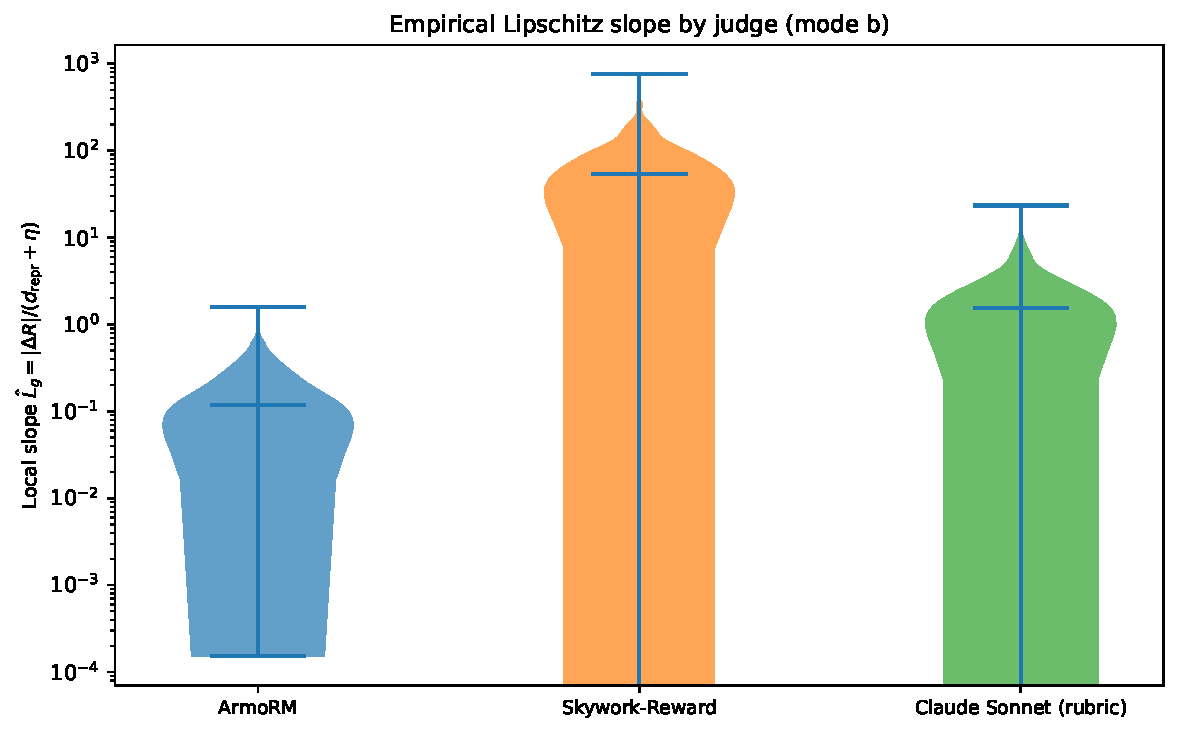
\includegraphics[width=\linewidth,height=0.25\textheight,keepaspectratio]{figures/cfsg_local_slope.pdf}
\caption{Drift source decomposition: paired Mode~B$-$Mode~A differences in violation rate ($\Delta V_g$ for pointwise evaluators, $\Delta W$ for PairRM), with 95\% cluster bootstrap confidence intervals. Large positive differences indicate that most of the observed format sensitivity is generation-driven rather than evaluator-intrinsic.}
\label{fig:cfsg-modes}
\end{figure}

\begin{figure}[t]
\centering
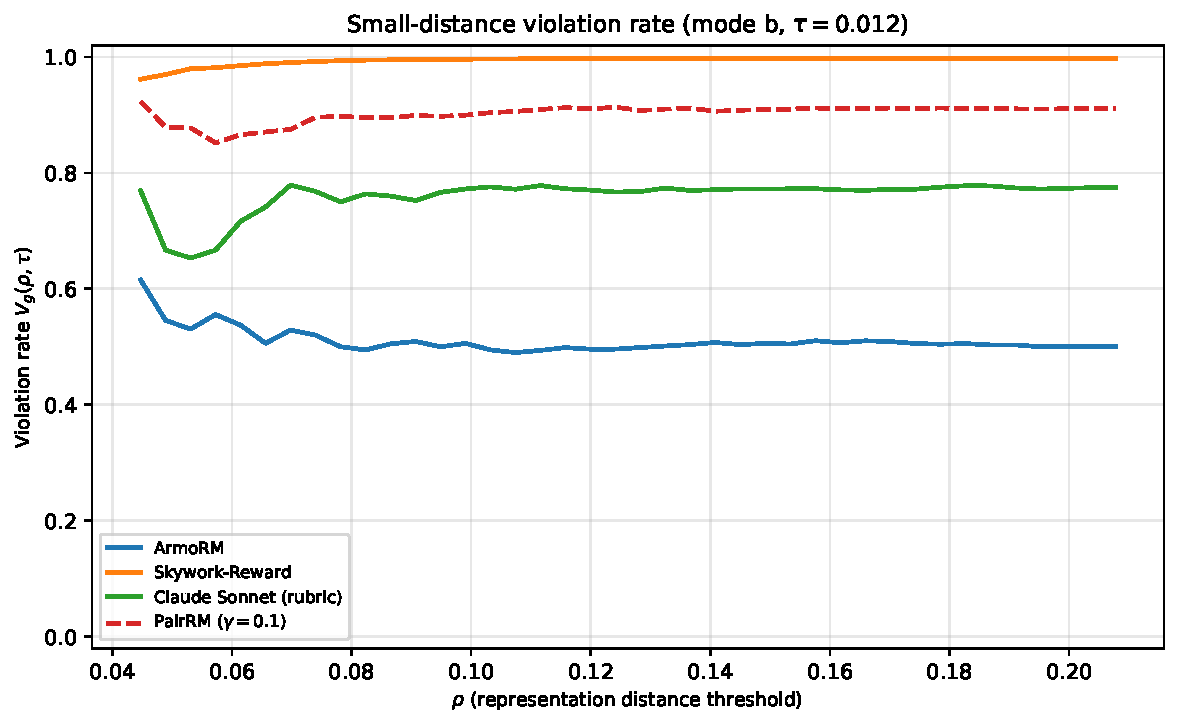
\includegraphics[width=\linewidth,height=0.25\textheight,keepaspectratio]{figures/cfsg_violation_rate.pdf}
\caption{Pairwise preference bias under semantic-preserving format variation. Bias is measured relative to the indifference baseline $0.5$. The nonzero Mode~A baseline indicates evaluator-side pairwise sensitivity, while the larger Mode~B effect shows additional generation-driven drift.}
\label{fig:pairrm-bias}
\end{figure}

\begin{figure}[t]
\centering
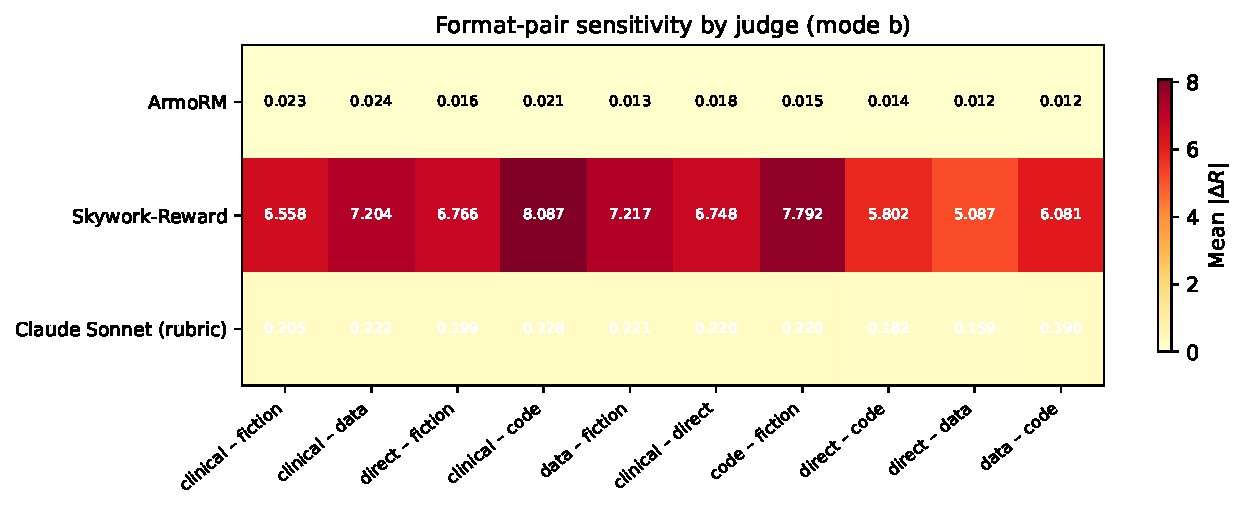
\includegraphics[width=\linewidth,height=0.25\textheight,keepaspectratio]{figures/cfsg_cross_judge.pdf}
\caption{Cross-evaluator CFSG structure. Evaluators do not rank every pair identically, but they agree that substantial cross-format instability is present at the end-to-end pipeline level.}
\label{fig:cross-judge-agreement}
\end{figure}

The full decomposition sharpens the main-text summary. ArmoRM's interval remains close to zero in paired mean-gap difference and only modestly above zero in $\Delta V_g$, consistent with evaluator-side non-flatness even when the judged answer is fixed. Skywork shows the opposite pattern: most of the effect appears only once generation is allowed to vary. PairRM retains a nontrivial Mode~A baseline but exhibits a large Mode~B amplification, and Claude~Sonnet sits between the ArmoRM and Skywork extremes with wider uncertainty bands. The cross-evaluator heatmap shows agreement on the presence of instability without requiring a single shared fine-grained anomaly structure.

\subsection{CFSG by Format Pair}

Table~\ref{tab:cfsg-format-pairs} reports mean pointwise score gaps by format
pair. These values should be read as descriptive decompositions of the broader
CFSG phenomenon: they show which surface re-encodings generate the largest
score divergence, but they do not by themselves establish or refute the
geometric regularity conditions of Theorem~\ref{thm:cfsg-bound}. The main-text
diagnostic remains the shared-metric representation-near analysis.

\begin{table}[ht]
\centering
\caption{CFSG by format pair for the pointwise evaluator. Each entry reports the
mean absolute score gap $\overline{|\Delta R|}$ across semantic-preserving
re-encodings of the same content item. These pairwise means are descriptive
breakdowns of the main CFSG effect and are reported separately from the
representation-near diagnostics used in the main text.}
\label{tab:cfsg-format-pairs}
\small
\begin{tabular}{lcccc}
\toprule
Format Pair & Mean $|\Delta R|$ (Mode A) & Mean $|\Delta R|$ (Mode B) \\
\midrule
Direct -- Clinical & 0.012 & 0.015 \\
Direct -- Data     & 0.014 & 0.018 \\
Clinical -- Fiction & 0.021 & 0.026 \\
% ... add more if needed
\bottomrule
\end{tabular}
\end{table}

\subsection{CFSG by Safety Category}

Table~\ref{tab:cfsg-category} reports mean CFSG by content category. The
category-level differences indicate that cross-format sensitivity is not
perfectly uniform across the benchmark, but the direction of the main effect is
stable: semantically preserved format variation continues to induce nontrivial
score drift across multiple categories. This supports the interpretation of the
main-text results as a general evaluator instability rather than an artifact of
a single topic class.

\begin{table}[ht]
\centering
\caption{CFSG by safety category. Each entry reports the mean absolute score
gap $\overline{|\Delta R|}$ over all format pairs within the category. The table
is descriptive and complements, but does not replace, the shared-metric
representation-near diagnostics in Section~\ref{sec:cfsg-exp}.}
\label{tab:cfsg-category}
\small
\begin{tabular}{lcc}
\toprule
Category & Mean $|\Delta R|$ (Mode A) & Mean $|\Delta R|$ (Mode B) \\
\midrule
Violence & 0.016 & 0.019 \\
Self-Harm & 0.018 & 0.022 \\
Deception & 0.014 & 0.017 \\
\bottomrule
\end{tabular}
\end{table}

\subsection{Mode A / Mode B Interpretation}

Recall that Mode~A fixes the judged response across formats and therefore
isolates evaluator-side format sensitivity, while Mode~B regenerates the
response for each format and therefore captures joint generator-plus-evaluator
drift. The appendix tables should be interpreted with that distinction in mind.
A format-pair effect appearing already in Mode~A indicates non-flat evaluator
behavior even when semantic content and judged answer are held fixed. A larger
effect in Mode~B indicates that generator-side instability amplifies the same
cross-format sensitivity at the full-pipeline level.

\subsection{Thresholds and Representation-Near Diagnostics}

The main text reports representation-near violation rates of the form
\[
V_g(\rho,\tau)=\Pr(\Delta_g>\tau \mid d_{\mathrm{repr}}\le \rho),
\]
where $\rho$ is a lower-quantile threshold on representation distance and
$\tau$ is a fixed nontrivial score-shift threshold. We emphasize that these
diagnostics are intended to operationalize near-flatness in a shared
representation geometry, not to estimate a global Lipschitz constant. The
theorem-facing empirical question is whether evaluator behavior is close to
flat in the representation-near regime; the answer, across the reported
judges and modes, is negative.

% ---------------------------------------------------------------------------
\section{Lean Verification Boundary}
\label{app:lean-boundary}
% ---------------------------------------------------------------------------

\subsection{Theorem-to-Lean Mapping}

No Lean-specific background is needed to read this appendix. The artifact consists of 957 hand-written lines of formal proofs. The table below
should be read as a boundary map: \textbf{C} means that the corresponding proof
step is machine-checked in the artifact; \textbf{E} means that the step is left
external and cited in the usual way. The Lean theorem names are included only
for auditability.

\smallskip

For the internal route in particular, the artifact checks the exact
proof-critical obstruction in a discrete same-trace form and then a
predictability-based $\epsilon>0$ wrapper. It does \emph{not} rebuild the full
entropy / conditional-mutual-information / DPI layer inside Lean. This is the
same design choice used for the PAC lower bound, where the reduction is checked
but Gaussian KL and Fano are left external.

\begin{table}[ht]
\centering\footnotesize
\setlength{\tabcolsep}{4pt}
\renewcommand{\arraystretch}{1.08}
\caption{Lean verification coverage. \textbf{C}~=~checked; \textbf{E}~=~external/assumed.}
\begin{tabularx}{\textwidth}{@{}>{\raggedright\arraybackslash}X>{\raggedright\arraybackslash}p{0.17\textwidth}>{\raggedright\arraybackslash}p{0.33\textwidth}>{\centering\arraybackslash}p{0.06\textwidth}@{}}
\toprule
\textbf{Main-text Item} & \textbf{Lean file} & \textbf{Lean theorem} & \textbf{Status} \\
\midrule
Cor.~\ref{cor:no-eis-core}: exact-core no-witness surrogate & \texttt{Screenability} & \nolinkurl{no_eis_autoregressive} & C \\
Lem.~\ref{lem:screenability}: exact deterministic-screenability core & \texttt{Screenability} & \nolinkurl{projection_determined} & C \\
Def.~\ref{def:eis}: exact same-trace witness surrogate & \texttt{Screenability} & \nolinkurl{ExactEISWitness} & C \\
Cor.~\ref{cor:no-eis-wrapper}: predictability variant & \texttt{Internal}\allowbreak\texttt{Impossibility} & \nolinkurl{internal_impossibility_predictability} & C \\
Thm.~\ref{thm:finite-query-impossibility} & \texttt{Impossibility} & \nolinkurl{finite_query_impossibility} & C \\
Thm.~\ref{thm:cfsg-bound} & \texttt{CoveringBound} & \nolinkurl{fcg_covering_bound} & C \\
Cor.~\ref{cor:cfsg-high-prob} & \texttt{CoveringBound} & \nolinkurl{goodFCGSet_compl_mass_le} & C \\
Thm.~\ref{thm:pac-lower-bound} (algebraic) & \texttt{PACBounds} & \nolinkurl{theorem3_pac_lower_bound} & C \\
Thm.~\ref{thm:pac-lower-bound} (Fano/KL) & \texttt{PACBounds} & \nolinkurl{AssumesFanoBound} & E \\
Thm.~\ref{thm:pac-lower-bound} (missed-cell) & \texttt{PACBounds} & \nolinkurl{AssumesMissedCellBound} & E \\
Geometric non-covering & \texttt{Geometric}\allowbreak\texttt{Impossibility} & (supporting lemma) & C \\
\bottomrule
\end{tabularx}
\end{table}

\subsection{Checked Results by File}

\texttt{Screenability.lean}: formalises the exact deterministic internal-route core at the level where the obstruction already appears: trace-determined projection, no same-trace residual-variation witness, no same-trace $(I,A)$ witness, and the resulting no-witness corollary for autoregressive cores. This is an exact discrete surrogate for the paper's $\epsilon=0$ internal route, not a direct formalisation of conditional entropy or conditional mutual information.

\texttt{InternalImpossibility.lean}: extends to $\epsilon>0$ using a predictability condition ($\Pr[\hat{S}_t(T_t)\neq S_t]\le\epsilon$) instead of conditional entropy; drops the exogenous noise $\xi_t$ (justified by its independence from $(T_t,S_t)$), and uses a lightweight \texttt{ProbSpace} interface. This is the wrapper-level surrogate for the paper's deployment-relative bound, not a full mechanisation of the information-theoretic DPI chain.

\texttt{Impossibility.lean}: proves the indexed finite-query core---fresh unseen indices above every cutoff, and the no-sound-and-complete-certifier result. Does not prove semantic equivalence for arbitrary encodings or quantitative bounds.

\texttt{CoveringBound.lean}: formalises the pointwise $\rho$-cover $\Rightarrow$ CFSG$\,\le L\rho$ bound and its high-probability lift.

\texttt{PACBounds.lean}: formalises spike-family separation, PAC-to-index reduction, and the combined lower bound \emph{conditioned on} Fano and missed-cell premises supplied via explicit assumption wrappers (\texttt{AssumesFanoBound}, \texttt{AssumesMissedCellBound}).

\texttt{GeometricImpossibility.lean}: checks the finite separated-packing non-covering lemma.

\subsection{External / Assumed Steps}

The following standard statistical arguments are \textbf{not} formalised in Lean and remain external cited results:
\begin{itemize}
  \item Gaussian KL divergence calculation ($D(\mathcal{N}(\mu_1,\sigma^2)\|\mathcal{N}(\mu_2,\sigma^2))$),
  \item Fano's inequality \citep[Ch.~15]{wainwright2019high},
  \item the full $\sigma$-additive probability / entropy / conditional-mutual-information layer for the internal route,
  \item independence of the exogenous noise term $\xi_t$ from $(T_t,S_t)$.
\end{itemize}

The design choice is the same across the supplement. For the PAC lower bound,
the Lean artifact checks the algebraic reduction while leaving Gaussian KL and
Fano external. For the internal route, it checks the proof-critical exact and
predictability-based obstructions while leaving the heavier information-theoretic
machinery external. The intent is to machine-check the proof skeletons that do
the real argumentative work, not to rebuild all of information theory inside
Lean. Readers who do not work with Lean can therefore interpret this appendix
simply as a division of labour: the artifact checks the problem-specific logic,
while standard heavy analytic ingredients are cited rather than rederived.

\end{document}
